\section{2007 - PHYSICS 2A ALTERNATIVE A PRACTICAL}

\begin{enumerate}
\item[1.] The aim of this experiment is to determine the mass of a given object ``B'', and the constant of the spring provided.

\begin{center}
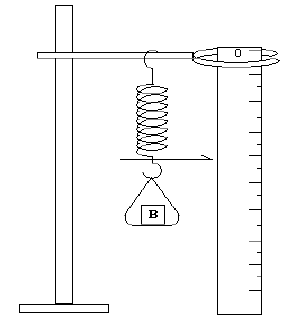
\includegraphics[width=7cm]{./img/2007-1-alt.png}
\end{center}

\begin{itemize}
\item[]
\begin{itemize}
\item[(i)] Set up the apparatus as shown in Fig. 1 with zero mark of the metre-rule at the top of the rule and record the scale reading by the pointer, $S_0$.
\item[(ii)] Place the object ``B'' and standard weight (mass) W equal to 20 g in the pan and record the new pointer reading $S_1$. Calculate the extension, $e = S_1 - S_0$ in cm.
\item[(iii)] Repeat the procedure in (ii) above with W = 40 g, 60 g, 80 g and 100 g.
\end{itemize}
\item[(a)] Record your results in tabular form as shown below:\\
Table of Results:

\begin{tabular}{|p{2cm}|p{3cm}|p{3cm}|p{3cm}|}\cline{1-1}
\multicolumn{1}{|p{2cm}|}{$S_0 = $}&\multicolumn{2}{c}{} & \multicolumn{1}{p{2.5cm}}{} \\ \hline
\multicolumn{1}{|c|}{Mass} & \multicolumn{1}{c|}{Force, F (N)} & \multicolumn{1}{c|}{Pointer reading $S_1$} & \multicolumn{1}{c|}{Extension}\\
\multicolumn{1}{|c|}{(kg)} & \multicolumn{1}{c|}{} & \multicolumn{1}{c|}{(cm)} & \multicolumn{1}{c|}{$= S_1 - S_0$ (cm)}\\ \hline
\multicolumn{1}{|c|}{0} & \multicolumn{1}{c|}{} & \multicolumn{1}{c|}{} & \multicolumn{1}{c|}{}\\ 
\multicolumn{1}{|c|}{0.02} & \multicolumn{1}{c|}{} & \multicolumn{1}{c|}{} & \multicolumn{1}{c|}{}\\ 
\multicolumn{1}{|c|}{0.04} & \multicolumn{1}{c|}{} & \multicolumn{1}{c|}{} & \multicolumn{1}{c|}{}\\ 
\multicolumn{1}{|c|}{0.06} & \multicolumn{1}{c|}{} & \multicolumn{1}{c|}{} & \multicolumn{1}{c|}{}\\ 
\multicolumn{1}{|c|}{0.08} & \multicolumn{1}{c|}{} & \multicolumn{1}{c|}{} & \multicolumn{1}{c|}{}\\ 
\multicolumn{1}{|c|}{0.10} & \multicolumn{1}{c|}{} & \multicolumn{1}{c|}{} & \multicolumn{1}{c|}{}\\ \hline
\end{tabular}
\item[(b)] Plot graph of Force F (vertical axis) against extension $e$ (horizontal axis).
\item[(c)] Use your graph to evaluate
\begin{itemize}
\item[(i)] mass of B
\item[(ii)] spring constant, K, given that force, extension, constant and weight of B are related as follows:\\
F = K$e$ - B
\end{itemize}
\end{itemize}

\end{enumerate}
\flushright \textbf{(25 marks)}



\begin{enumerate}
\item[2.] The aim of this experiment is to find the refractive index of a glass block. Proceed as following:\\[10pt]

Place the given glass block in the middle of the drawing paper on the drawing board. Draw lines along the upper and lower edge of the glass block. Remove the glass block and extend the line you have drawn. Represent the ends of those line segments as SS$^1$ and TT$^1$. Draw the normal NN$^1$ to the parallel lines SS$^1$ and TT$^1$ as shown in Fig. 2(a).

\begin{center}
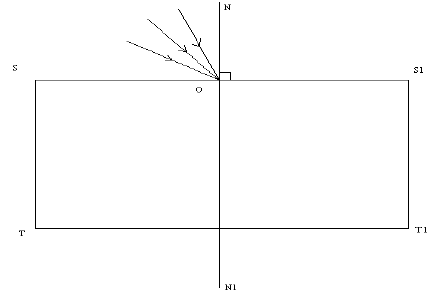
\includegraphics[width=8cm]{./img/2007-2a-alt.png}
\end{center}

Draw five evenly spaced lines from O to represent incident rays at different angles of incidence (10$^\circ$, 20$^\circ$, 30$^\circ$, 40$^\circ$ and 50$^\circ$ from the normal). Replace the glass block carefully between SS$^1$ and TT$^1$. Stick two pins P$_1$ and P$_2$ as shown in Fig. 2(b) as far apart as possible along one of the lines drawn to represent an incident ray. Locate an emergent ray by looking through the block and stick pins P$_3$ and P$_4$ exactly in line with images I$_1$ and I$_2$ of pins P$_1$ and P$_2$. Draw the emergent ray and repeat the procedure for all the incident rays you have drawn. Finally draw in the corresponding refracted rays.\\[10pt]

NOTE: The drawing paper should be handed in together with other answer sheets.

\begin{center}
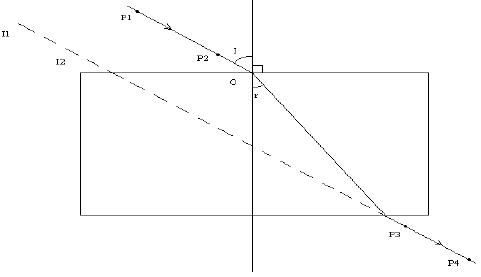
\includegraphics[width=10cm]{./img/2007-2b-alt.png}
\end{center}

\begin{itemize}
\item[(a)] Record the angles of incidence I and the measured corresponding angles of refraction ``r'' in a table. Your table of results should include the values of $\sin$ I and $\sin$ r.
\item[(b)] Plot the graph of $\sin$ I (vertical - axis) against $\sin$ r (horizontal - axis).
\item[(c)] Determine the slope of the graph.
\item[(d)] What is the refractive index of the glass block used?
\item[(e)] Mention any sources of errors in this experiment.
\end{itemize}

\end{enumerate}
\flushright \textbf{(25 marks)}


\begin{enumerate}
\item[3.] The aim of this experiment is to determine the potential fall along a uniform resistance wire carrying a steady current.\\[10pt]

Proceed as follows:

\begin{center}
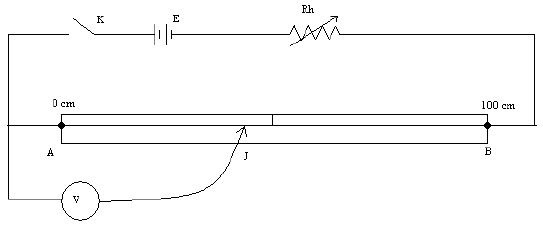
\includegraphics[width=12cm]{./img/2007-3-alt.png}
\end{center}

Connect up the circuit as shown in Fig. 3. Adjust the rheostat so that when the sliding contact J is near B, and the key is closed the voltmeter V indicates an almost full scale deflection. Do not alter the rheostat again.\\

Close key K and make contact with J, so that AJ = 10 cm. Record the potential different V volts between A and J as registered on the voltmeter.\\

Repeat this procedure for AJ = 20 cm, 30 cm, 50 cm and 70 cm.

\begin{itemize}
\item[(a)] Tabulate your results for the values of AJ and V.
\item[(b)] Plot a graph of V (vertical axis) against AJ (horizontal axis).
\item[(c)] Calculate the slope of the graph.
\item[(d)] What is your comment on the slope?
\item[(e)] State any precautions on the experiment.
\end{itemize}

\end{enumerate}
\flushright \textbf{(25 marks)}
\flushleft